\chapter{Queue Results}

\section{Cache Misses}

The results are collected by evaluating the Multi-Thread Singletons Test with each thread running 10M transactions under the profiling tool Performance Events for Linux (\texttt{perf}). The sampling period is set to 1000, meaning that every 1000th cache miss is recorded.

In these figures, we report the number of cache misses reported by perf (approximately 1/1000 of the actual number of cache misses.)

\begin{figure}[H]
    \centering
    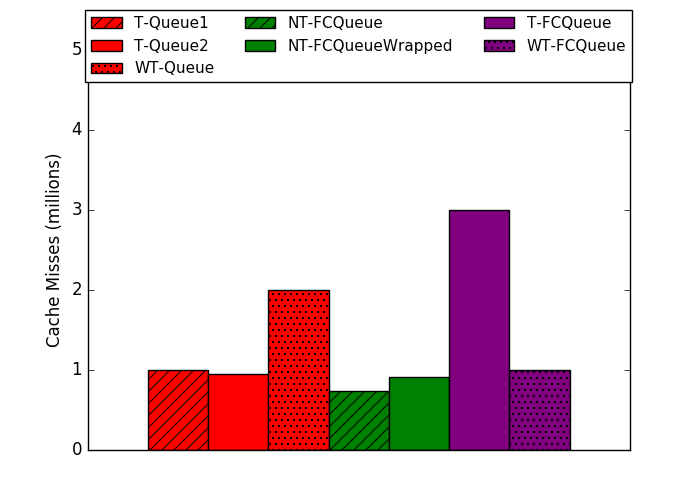
\includegraphics[width=\textwidth]{fcqueues/cm.png}
    \caption{Queue Cache Misses}
\label{fig:cm_queues}
\end{figure}

\section{Push-Pop Test Results}

\begin{figure}[H]
    \centering
    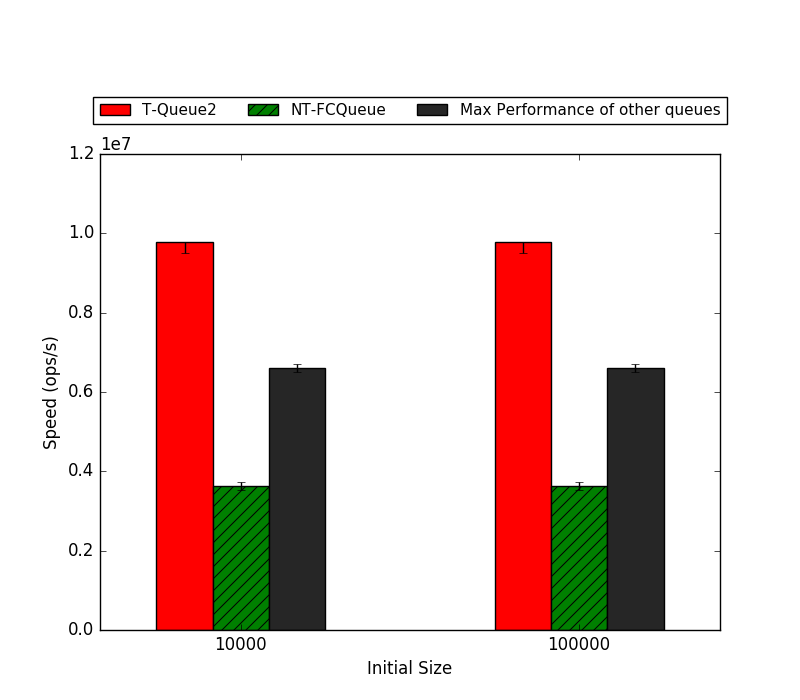
\includegraphics[width=\textwidth]{concurrent/Q:PushPop.png}
    \caption{Push-Pop Test: Concurrent, Non-transactional Queues}
    \label{fig:concurrentqs_pushpop}
\end{figure}

\begin{figure}[H]
    \centering
	\begin{minipage}{0.45\textwidth}
	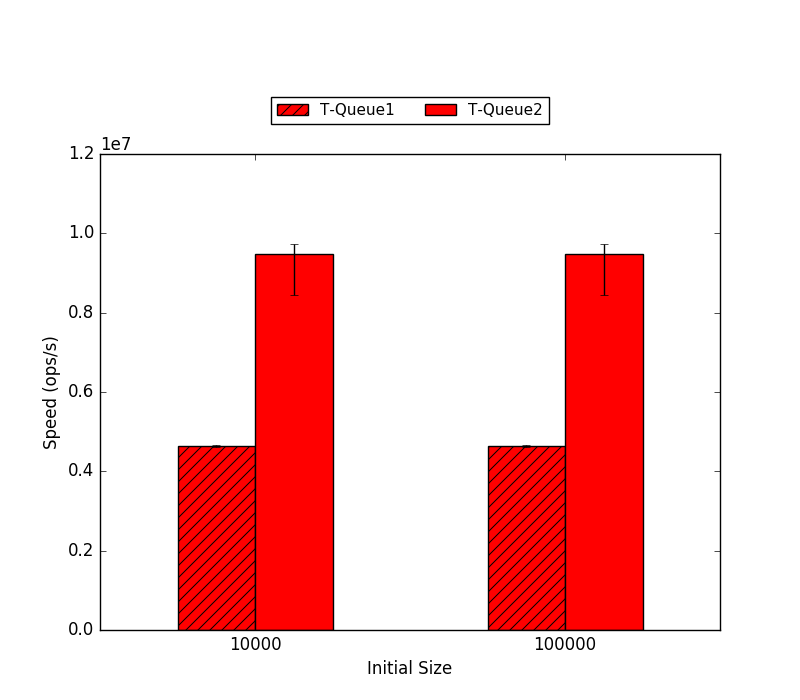
\includegraphics[width=\textwidth]{fcqueues/stoQ:PushPop.png}
	\end{minipage}
	\begin{minipage}{0.45\textwidth}
		\begin{tabular}{|c|c|c|}
\hline
\multirow{2}{*}{Queue} & \multicolumn{2}{c|}{Initial Size}\\\cline{2-3}& \qquad 10000 \qquad\quad & \qquad 100000\qquad\quad\\
\hline
\hline
T-QueueO & 0.00001 & 0.00001\\
T-QueueP & 1.54560 & 1.60886\\
\hline\end{tabular}

	\end{minipage}
    \caption{Push-Pop Test: T-Queue1 vs. T-Queue2}
    \label{fig:stoqs_pushpop}
\end{figure}

\begin{figure}[H]
    \centering
	\begin{minipage}{0.45\textwidth}
    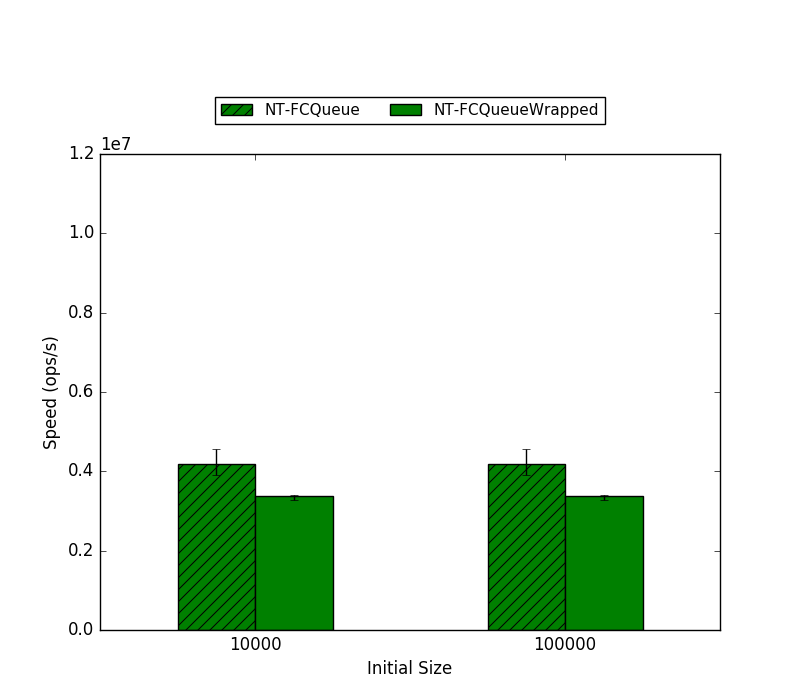
\includegraphics[width=\textwidth]{fcqueues/ntQ:PushPop.png}
	\end{minipage}
	\begin{minipage}{0.45\textwidth}
    \begin{tabular}{|c|c|c|}
\hline
\multirow{2}{*}{Queue} & \multicolumn{2}{c|}{Initial Size}\\\cline{2-3}& \qquad 10000 \qquad\quad & \qquad 100000\qquad\quad\\
\hline
\hline
NT-FCQueue & 0.00000 & 0.00000\\
\hline\end{tabular}

	\end{minipage}
    \caption{Push-Pop Test: NT-FCQueueWrapped vs. NT-FCQueue}
    \label{fig:ntqs_pushpop}
\end{figure}

\begin{figure}[H]
    \centering
	\begin{minipage}{0.45\textwidth}
    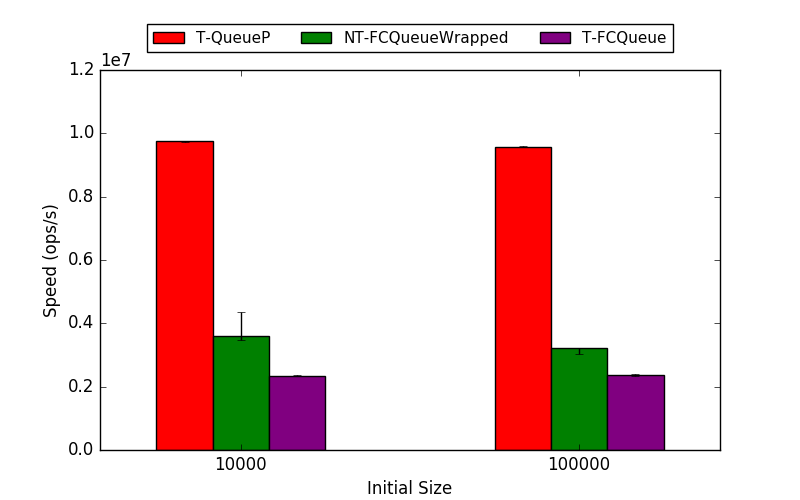
\includegraphics[width=\textwidth]{fcqueues/tQ:PushPop.png}
	\end{minipage}
	\begin{minipage}{0.45\textwidth}
    \begin{tabular}{|c|c|c|}
\hline
\multirow{2}{*}{Queue} & \multicolumn{2}{c|}{Initial Size}\\\cline{2-3}& \qquad 10000 \qquad\quad & \qquad 100000\qquad\quad\\
\hline
\hline
T-QueueP & 1.54560 & 1.60886\\
T-FCQueue & 0.62494 & 1.62620\\
\hline\end{tabular}

	\end{minipage}
    \caption{Push-Pop Test: T-FCQueue}
    \label{fig:tqs_pushpop}
\end{figure}

\begin{figure}[H]
    \centering
	\begin{minipage}{0.45\textwidth}
    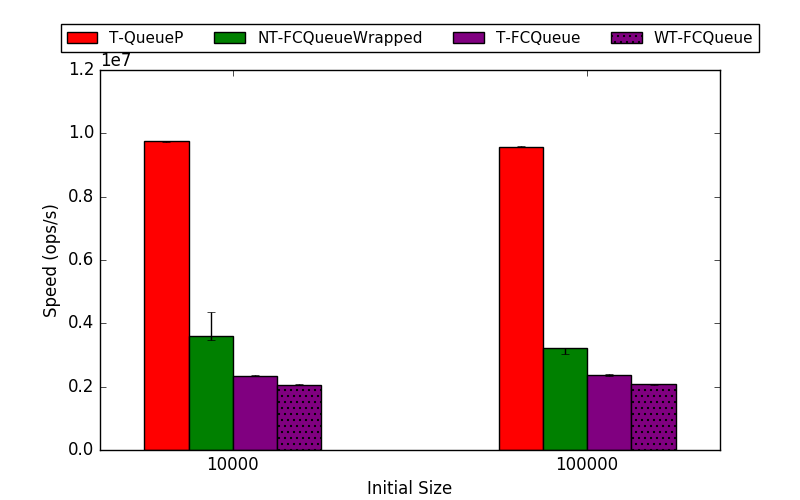
\includegraphics[width=\textwidth]{fcqueues/lpQ:PushPop.png}
	\end{minipage}
	\begin{minipage}{0.45\textwidth}
    \begin{tabular}{|c|c|c|}
\hline
\multirow{2}{*}{Queue} & \multicolumn{2}{c|}{Initial Size}\\\cline{2-3}& \qquad 10000 \qquad\quad & 100000\\
\hline
\hline
T-QueueP & 1.45435 & 1.45435\\
WT-Queue & 0.00000 & 0.00000\\
NT-FCQueueWrapped & 0.00000 & 0.00000\\
T-FCQueue & 0.00010 & 0.00010\\
WT-FCQueue & 0.00000 & 0.00000\\
\hline\end{tabular}

	\end{minipage}
    \caption{Push-Pop Test: WT-FCQueue}
    \label{fig:wtqs_pushpop}
\end{figure}

\section{Multi-Thread Singletons Test Results}

\begin{figure}[H]
\centering
    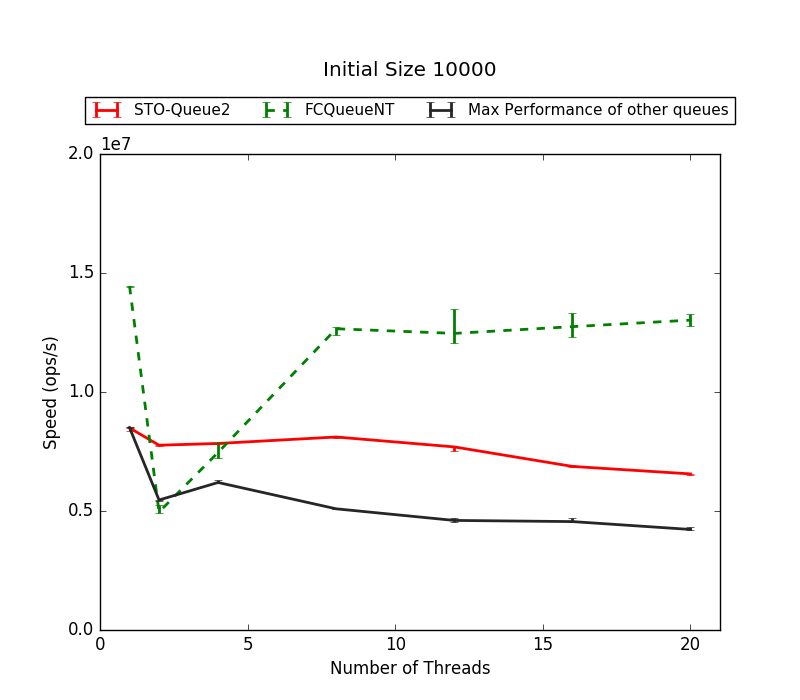
\includegraphics[width=0.5\textwidth]{concurrent/Q:RandSingleOps10000.png}
    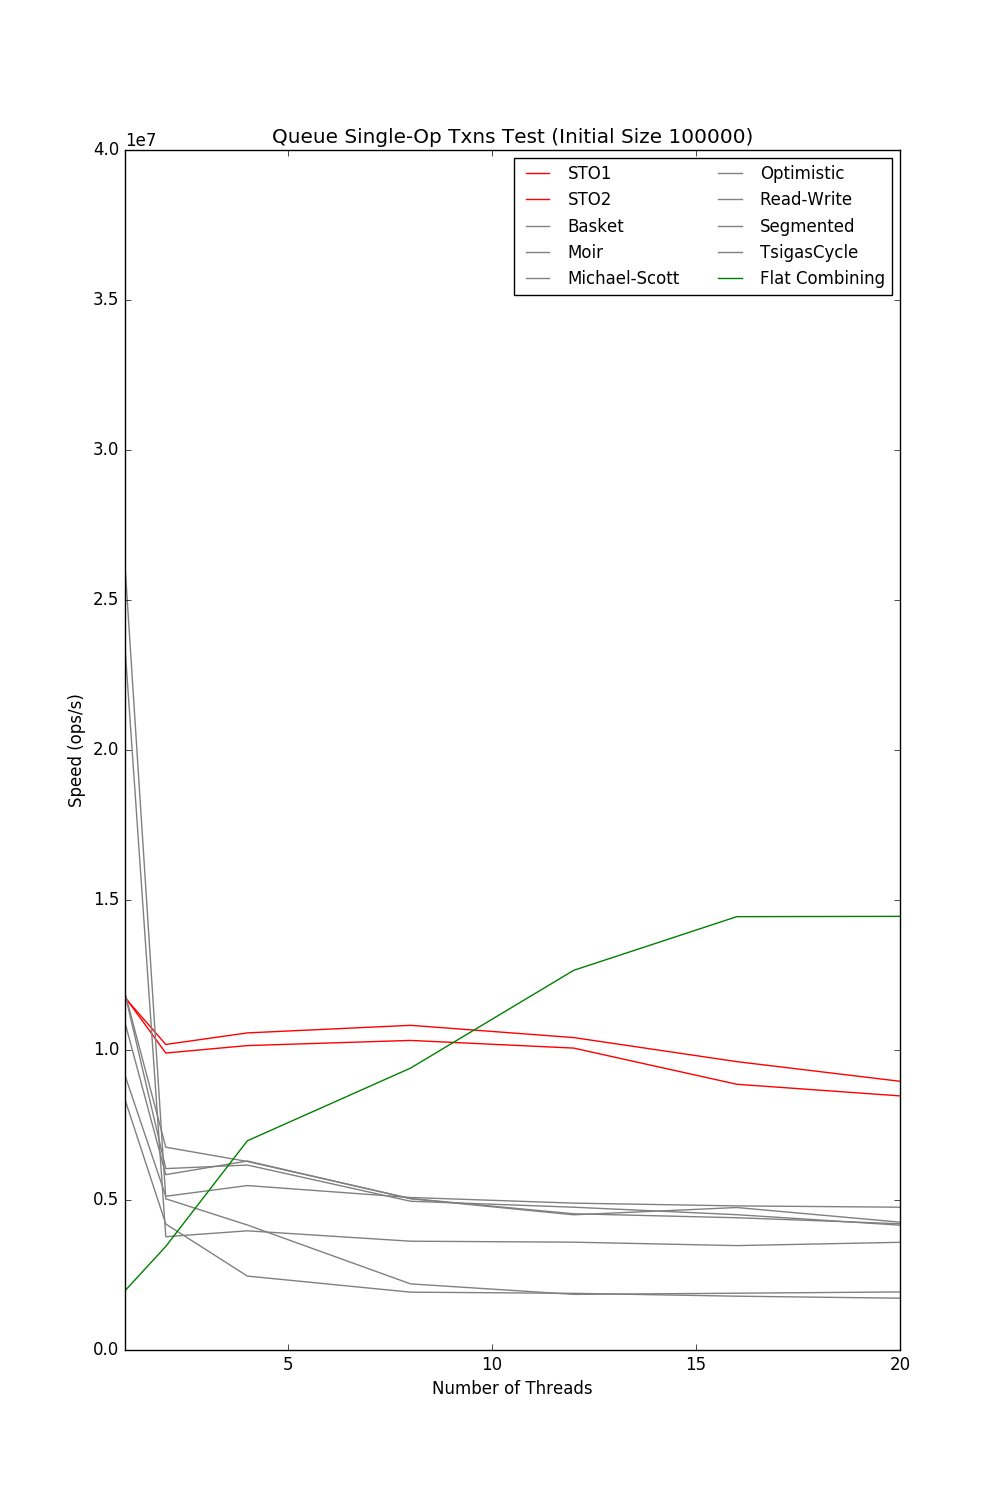
\includegraphics[width=0.5\textwidth]{concurrent/Q:RandSingleOps100000.png}
\caption{Multi-Thread Singletons Test: Concurrent, Non-transactional Queues}
\label{fig:concurrent_qs}
\end{figure}

\begin{figure}[H]
    \centering
    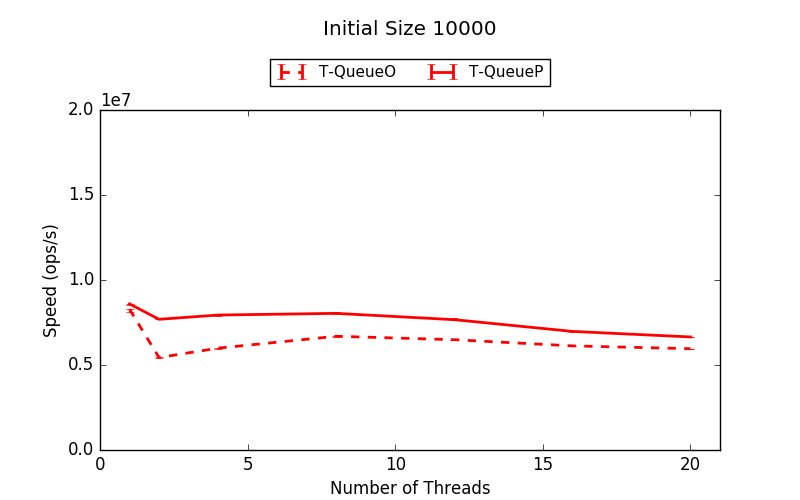
\includegraphics[width=0.5\textwidth]{fcqueues/stoQ:RandSingleOps10000.png}
    \begin{tabular}{|c|c|c|c|}
\hline
\multirow{2}{*}{Queue} & \multicolumn{3}{c|}{\#Threads}\\\cline{2-4}& \quad 4 & 12 & 20\\
\hline
\hline
T-QueueO & 9.55031 & 6.77475 & 6.38129\\
T-QueueP & 2.87497 & 2.29600 & 2.46225\\
\hline\end{tabular}

    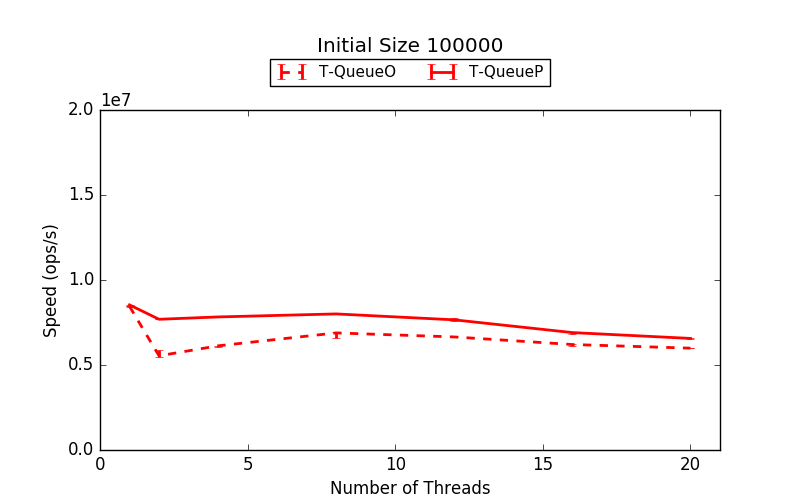
\includegraphics[width=0.5\textwidth]{fcqueues/stoQ:RandSingleOps100000.png}
    \begin{tabular}{|c|c|c|c|c|c|c|}
\hline
\multirow{2}{*}{Queue} & \multicolumn{6}{c|}{\#Threads}\\\cline{2-7}& 2 & 4 & 8 & 12 & 16 & 20\\
\hline
\hline
T-QueueO & 7.88767 & 10.67091 & 7.85545 & 7.54535 & 6.73918 & 6.48418\\
T-QueueP & 3.07026 & 2.70427 & 2.12894 & 2.22341 & 2.22941 & 2.27197\\
\hline\end{tabular}

\caption{Multi-Thread Singletons Test: T-Queue1 vs. T-Queue2}
\label{fig:stoqueues}
\end{figure}

\begin{figure}[H]
    \centering
    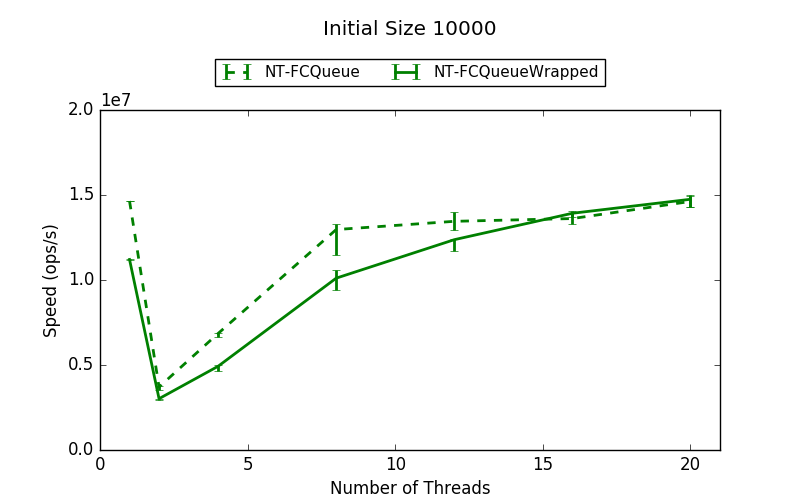
\includegraphics[width=0.5\textwidth]{fcqueues/ntQ:RandSingleOps10000.png}
    \begin{tabular}{|c|c|c|c|}
\hline
\multirow{2}{*}{Queue} & \multicolumn{3}{c|}{\#Threads}\\\cline{2-4}& \quad 4 & 12 & 20\\
\hline
\hline
NT-FCQueue & 0.00000 & 0.00000 & 0.00000\\
NT-FCQueueWrapped & 0.00000 & 0.00000 & 0.00000\\
\hline\end{tabular}

    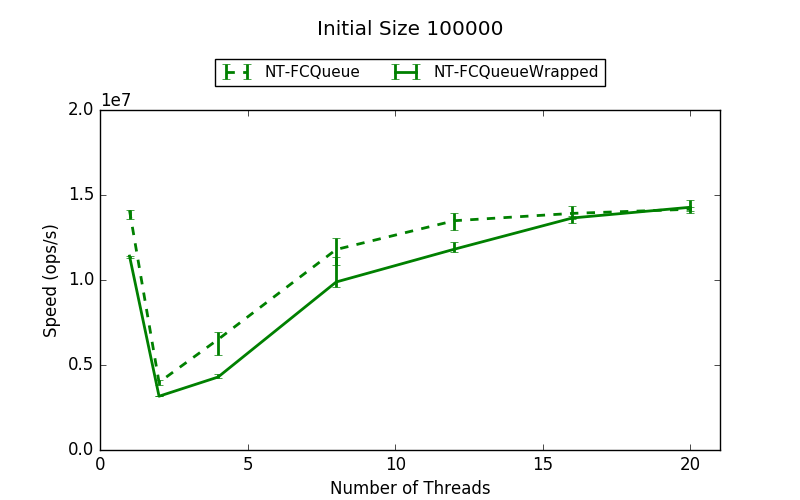
\includegraphics[width=0.5\textwidth]{fcqueues/ntQ:RandSingleOps100000.png}
    \begin{tabular}{|c|c|c|c|}
\hline
\multirow{2}{*}{Queue} & \multicolumn{3}{c|}{\#Threads}\\\cline{2-4}& \quad 4 & 12 & 20\\
\hline
\hline
NT-FCQueue & 0.00000 & 0.00000 & 0.00000\\
NT-FCQueueWrapped & 0.00000 & 0.00000 & 0.00000\\
\hline\end{tabular}

\caption{Multi-Thread Singletons Test: NT-FCQueueWrapped vs. NT-FCQueue}
\label{fig:ntqueues}
\end{figure}

\begin{figure}[H]
    \centering
    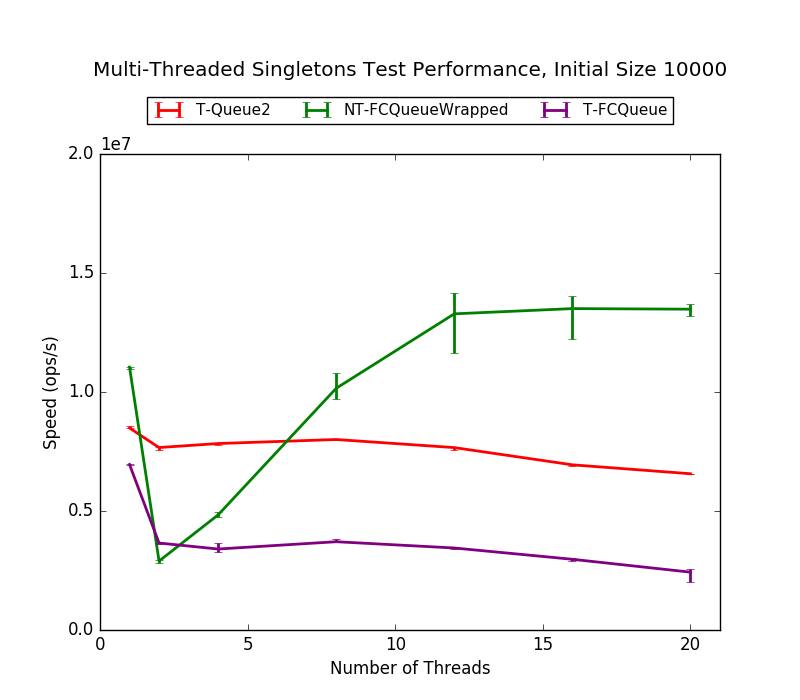
\includegraphics[width=0.5\textwidth]{fcqueues/tQ:RandSingleOps10000.png}
    \begin{tabular}{|c|c|c|c|c|c|c|}
\hline
\multirow{2}{*}{Queue} & \multicolumn{6}{c|}{\#Threads}\\\cline{2-7}& 2 & 4 & 8 & 12 & 16 & 20\\
\hline
\hline
T-QueueP & 3.25357 & 2.84958 & 2.23814 & 2.26892 & 2.31778 & 2.32787\\
T-FCQueue & 3.99773 & 6.08289 & 4.60842 & 4.78435 & 4.96070 & 5.33221\\
\hline\end{tabular}

    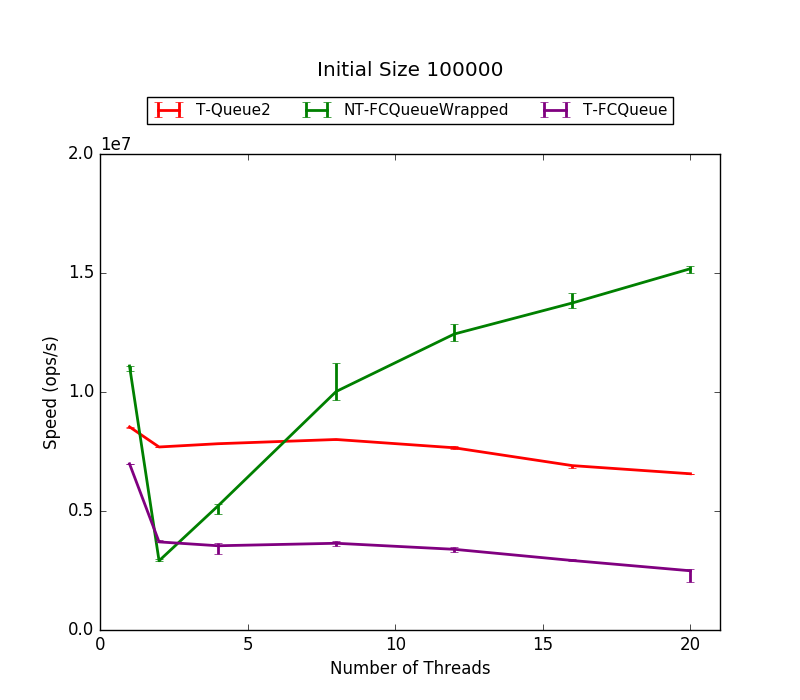
\includegraphics[width=0.5\textwidth]{fcqueues/tQ:RandSingleOps100000.png}
    \begin{tabular}{|c|c|c|c|}
\hline
\multirow{2}{*}{Queue} & \multicolumn{3}{c|}{\#Threads}\\\cline{2-4}& \quad 4 & 12 & 20\\
\hline
\hline
T-QueueP & 2.809 & 2.324 & 2.446\\
NT-FCQueueWrapped & 0.000 & 0.000 & 0.000\\
T-FCQueue & 4.436 & 3.521 & 4.207\\
\hline\end{tabular}

\caption{Multi-Thread Singletons Test: T-FCQueue}
\label{fig:tqueues}
\end{figure}

\begin{figure}[H]
    \centering
    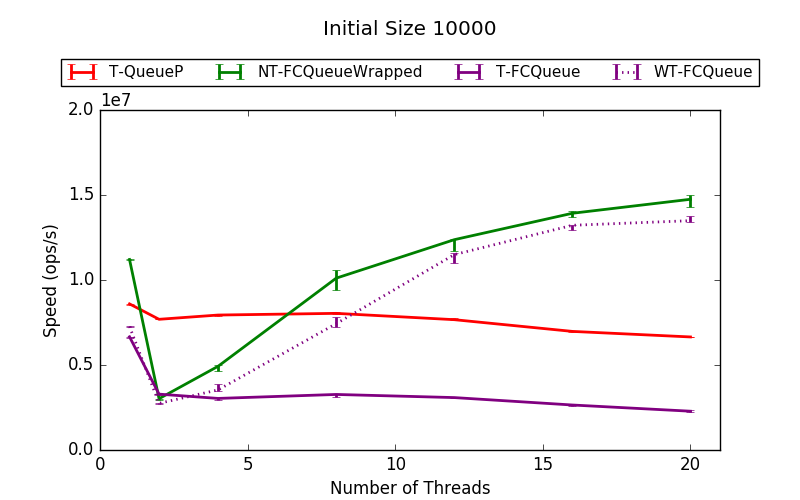
\includegraphics[width=0.5\textwidth]{fcqueues/lpQ:RandSingleOps10000.png}
    \begin{tabular}{|c|c|c|c|}
\hline
\multirow{2}{*}{Queue} & \multicolumn{3}{c|}{\#Threads}\\\cline{2-4}& \quad 4 & 12 & 20\\
\hline
\hline
T-QueueP & 2.84958 & 2.26892 & 2.32787\\
NT-FCQueueWrapped & 0.00000 & 0.00000 & 0.00000\\
T-FCQueue & 6.08289 & 4.78435 & 5.33221\\
WT-FCQueue & 0.00000 & 0.00000 & 0.00000\\
\hline\end{tabular}

    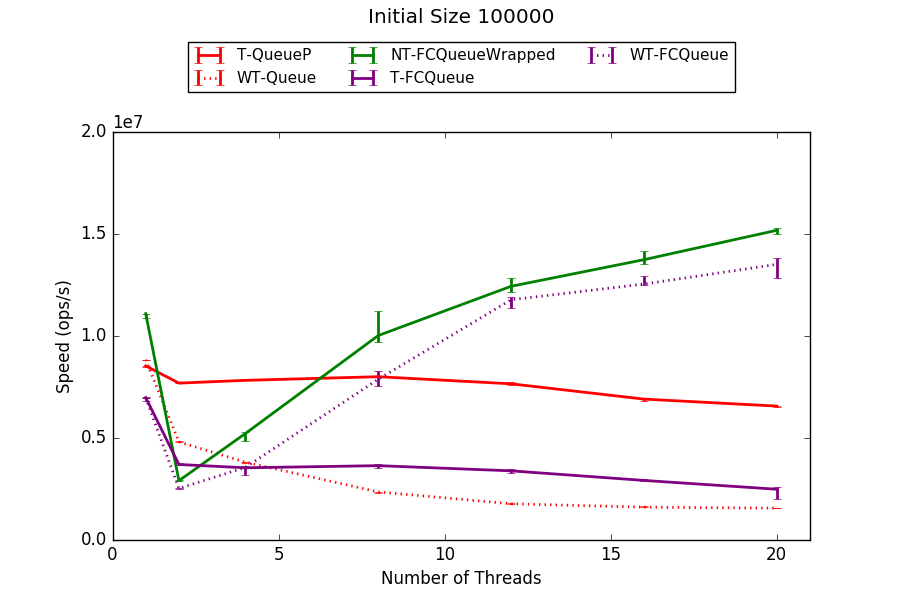
\includegraphics[width=0.5\textwidth]{fcqueues/lpQ:RandSingleOps100000.png}
    \begin{tabular}{|c|c|c|c|}
\hline
\multirow{2}{*}{Queue} & \multicolumn{3}{c|}{\#Threads}\\\cline{2-4}& \quad 4 & 12 & 20\\
\hline
\hline
T-QueueP & 2.809 & 2.324 & 2.446\\
WT-Queue & 16.600 & 59.998 & 71.140\\
NT-FCQueueWrapped & 0.000 & 0.000 & 0.000\\
T-FCQueue & 4.436 & 3.521 & 4.207\\
WT-FCQueue & 0.000 & 0.000 & 0.000\\
\hline\end{tabular}

\caption{Multi-Thread Singletons Test: WT-FCQueue}
\label{fig:wtqueues}
\end{figure}
